\chapter{Análisis y diseño de la solución}
\label{cha:AnalysisAndDesign}

En este capítulo se hablará del análisis y del diseño adoptado para resolver el problema de generar chatbots. Para ello, como se ha mencionado previamente, se ha definido un artefacto llamado SheetChat. En el Apartado \ref{sec:Requisitos} se hablará de los requisitos que ha de tener el artefacto que permita generar bots. En el Apartado \ref{sec:FeatureModel} se realizará el análisis de las funcionalidades que ha de tener SheetChat. Finalmente, en el Apartado \ref{sec:DataModel} se mostrará cual es el modelo de datos a definir para la generación de agentes conversacionales basados en hojas de cálculo.

\section{Requisitos}
\label{sec:Requisitos}

En la captura de requisitos hay dos vertientes que hay que tener en cuenta al tratarse de un software generador. Por un lado, hay que prestar atención que el generador cumpla con los requisitos funcionales y no funcionales. Por otro lado, hay que asegurar que el software generado también cumple con los requisitos preestablecidos.

Cabe destacar, tal y como se mencionaba en el Capítulo \ref{cha:Intro}, que el público objetivo que va a utilizar esta herramienta para el desarrollo va a ser gente con conocimientos de hojas de cálculo. Ellos mismos también serán los consumidores del chatbot que generen.

Dado que el usuario que utilizará SheetChat será un usuario con conocimientos para crear sus propias hojas de cálculo, se da por supuesto que éste \textbf{dispondrá de conocimientos de fórmulas matemáticas y de funciones de filtrado}. Es por ello que es apropiado proporcionarle un lenguaje que permita definir Chatbots con consultas y manipulación de datos más o menos potente.

Sin embargo, el usuario promedio de hojas de cálculo \textbf{no tiene conocimiento de los Chatbots}, qué es una API, un lenguaje de programación o procesamiento del lenguaje natural. Estos aspectos SheetChat deberá de abstraérselos al usuario.

Un aspecto fundamental es cómo se van a definir los Chatbots. La idea a largo plazo es que exista una herramienta gráfica que ayude a generar la sintaxis concreta de manera automática. Sin embargo dado el alcance de este trabajo, es conveniente \textbf{utilizar un lenguaje textual fácilmente legible por los seres humanos}.

En referencia al chatbot generado, este debe de cumplir con algunas características que se definen en el Capítulo \ref{cha:IntroChatbot}. Estas funcionalidades pueden resultar obvias, pero rara vez se cumplen en los chatbots que existen en la red, provocando que la usabilidad se merme \cite{Chan2016}.

\section{Modelo de características}
\label{sec:FeatureModel}

El diseño de la solución que se ha adoptado para la generación de chatbots o agentes conversacionales utilizando hojas de cálculo se divide en dos partes claramente diferenciadas. Esto es debido al objetivo que se ha presentado en los anteriores apartados, que es generar un chatbot para la consulta de datos extraídos de hojas de cálculo. Tal y como se puede observar en la Figura \ref{fig:FeatureModel}, por un lado hay que definir el origen de datos, los Sheet u hojas de cálculo. Por otro lado el cómo se consultan los datos, es decir, el chat o flujo de conversación que se define para obtener los resultados.


\begin{figure}[htb]
	\centering
	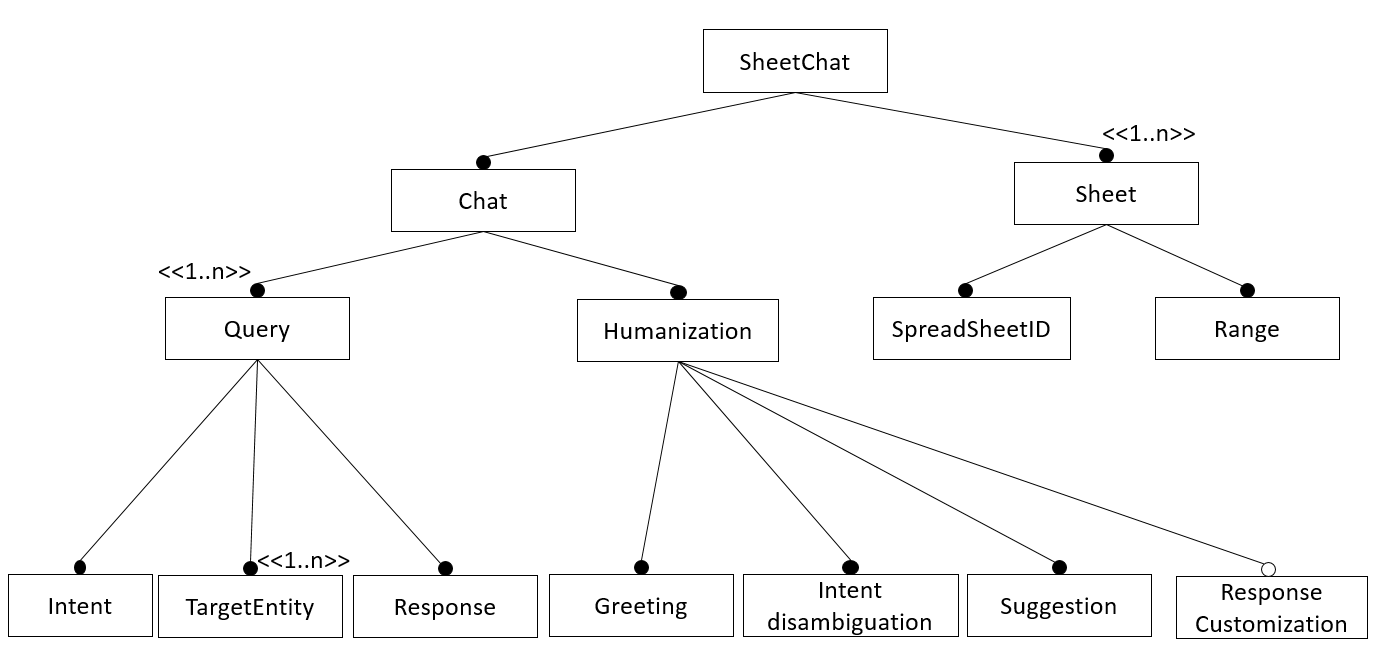
\includegraphics[width=0.8\textwidth]{./figs/FeatureModel.png}
	\caption{Modelo de características de SheetChat.}
	\label{fig:FeatureModel}
\end{figure}

En el Apartado \ref{sec:Sheet} se hablará sobre cómo se manejan las hojas de cálculo para su posterior consulta mediante un chatbot. En el Apartado \ref{sec:Chat} se describirá cómo se define un chatbot, el tipo de consultas (ver Apartado \ref{sec:Queries}) y el procedimiento para hacerlas. Asimismo se mostrará el cómo se realiza la humanización de un chatbot (ver Apartado \ref{sec:Humanization}), que permite mejorar la experiencia de usuario a la hora de conversar.

\subsection{Sheet}
\label{sec:Sheet}

La palabra Sheet de SheetChat hace referencia a las hojas de cálculo. Las hojas de cálculo son unas herramientas muy potentes que permiten, además de generar gráficas o trabajar con complejas funciones matemáticas, el almacenar datos en forma matricial (filas y columnas). Las hojas de cálculo están orientadas al análisis de datos y las bases de datos al almacenamiento de las mismas \cite{Philips2014}. Sin embargo, ambas almacenan datos basados en columnas y filas (o tuplas).

En el enfoque de nuestro trabajo, cada hoja de cálculo representa un conjunto de datos en forma de tabla. Al igual que sucede con los ficheros CSV, la primera fila es la cabecera de la tabla, donde se especifica cual es el nombre de cada columna (ver resaltado en azul de la Figura \ref{fig:SheetExample}). Las posteriores filas se traducen en tuplas que serán los datos a consultar.

Se pueden definir como origen de datos tantas hojas de cálculo se requieran para el chatbot. La única condición es que no tengan el mismo nombre la hoja de cálculo (resaltado en morado en la Figura \ref{fig:SheetExample}) y que los datos estén estructurados de una manera similar a lo que se puede observar en la Figura \ref{fig:SheetExample}.

\begin{figure}[htb]
	\centering
	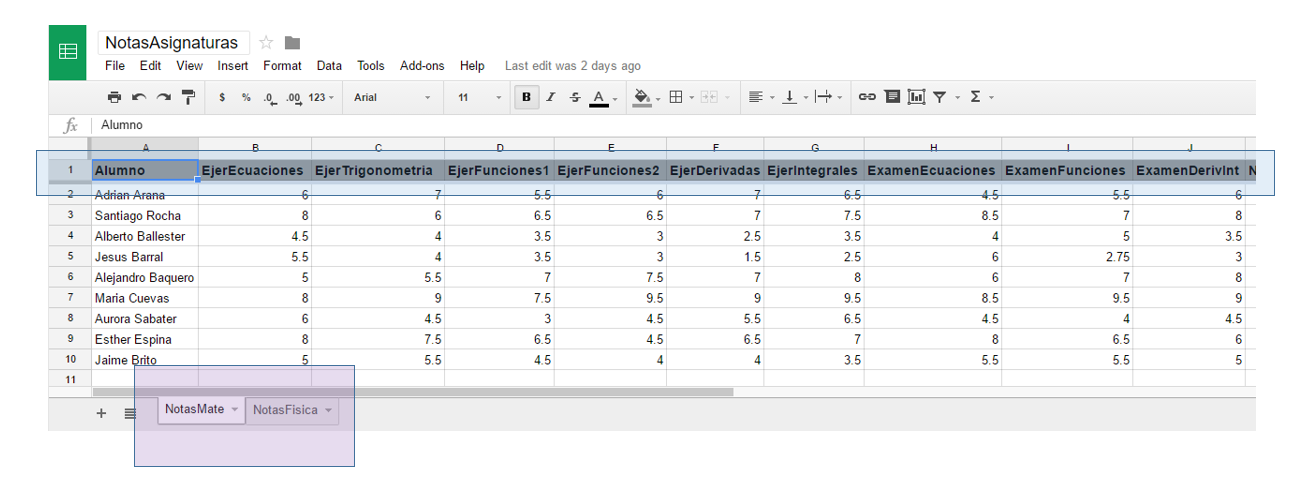
\includegraphics[width=1.1\textwidth]{./figs/SheetExample.png}
	\caption{Ejemplo de hoja de cálculo.}
	\label{fig:SheetExample}
\end{figure}

A la hora de definir un chatbot se pueden definir más de un origen de datos. En la tecnología utilizada hay que mencionar que se definen hojas de cálculo en Google SpreadSheet\footnote{Sitio web de Google SpreadSheets: \url{https://www.google.com/sheets/about/}}. La principal ventaja que ofrece esta tecnología es que los datos residen en la nube, lo que permite ser accedidos desde cualquier plataforma y en cualquier momento y siempre se dispondrá de la versión más actualizada de los datos a consultar.


Los datos de las hojas de cálculo serán adaptadas a una base de datos que permite consultas SQL. Esto permite que se puedan hacer consultas con cierto nivel de riqueza sobre las hojas de cálculo (funciones matemáticas y funciones de filtrado). Estas consultas se definen en el sistema de conversación de SheetChat en el Apartado \ref{sec:Queries}.


Cabe mencionar que SheetChat se encargará de hacer transparente la extracción (de Google SpreadSheets), transformación (a una base de datos en memoria) y actualización de los datos en tiempo real, tal y como se puede profundizar en el Apartado \ref{sec:AlaSQL}.

\subsection{Chat}
\label{sec:Chat}

El Chat de la palabra SheetChat hace referencia a la conversación que se ha de definir. La conversación es la interfaz de consultas a la hoja de cálculo que tendrá el usuario. Una conversación consiste en un proceso donde el usuario y el chatbot intercambian mensajes hasta que el usuario consigue resolver su duda u obtener la información que requiere. Una conversación puede consistir en un mensaje o más, dependerá en este caso de si el chatbot puede recabar todos los datos necesarios para proporcionar la respuesta.

El proceso de definir un Chat consta de dos partes. En el Apartado \ref{sec:Queries} se estudia qué son las consultas en SheetChat y en el Apartado \ref{sec:Humanization} se estudia las técnicas de humanización del bot que proporciona SheetChat.

\subsubsection{Consultas}
\label{sec:Queries}

Las consultas en SheetChat funcionan como el nexo entre una conversación y la hoja de cálculos. Definir adecuadamente una consulta permite que el usuario pueda preguntar por algo en concreto y el bot pueda obtener una respuesta rápida y fiable en la hoja de cálculo.

Una consulta, tal y como se puede observar en la Figura \ref{fig:FeatureModel} consta de tres partes, el Intent, las Entidades y la Respuesta. Definiendo estos tres aspectos, SheetChat es capaz de reconocer las preguntas que el usuario realice al chatbot y proporcionar una respuesta al mismo.

Para reconocer la pregunta que el usuario hace se definen dos aspectos, el Intent y las Entidades:
\begin{itemize}
	\item El \textbf{Intent} representa la intención del usuario. ``Saber si un alumno ha aprobado una asignatura'', ``Saber a qué hora parte el próximo tren a un destino concreto'' o ``Informarse sobre los restaurantes con comida de un tipo concreto'' son intenciones de usuario. Los Intents esperan como respuesta un concepto muy concreto, sin embargo la manera de preguntar sobre el mismo Intent puede ser bastante diferente: ``Ha aprobado un alumno concreto la asignatura de Inglés?'' o ``Debe un alumno concreto presentarse a la segunda convocatoria de Inglés?'' hacen referencia al mismo Intent. Sin embargo, para un sistema computacional es complejo desambiguar esto. En el Apartado \ref{sec:Humanization} se profundiza en cómo resolver esta problemática.
	\item Las \textbf{Entidades} representan los elementos u objetos de un contexto determinado. En las preguntas de ejemplo definidas anteriormente, no hacían referencia a un objeto del contexto. En la pregunta ``Ha aprobado un alumno concreto la asignatura de Inglés?'' no se especificaba el nombre de a qué alumno se refiere el usuario. Las entidades vienen a representar en este contexto a los alumnos, Miguel, Maria, Juan,... En las consultas las entidades hacen la función de filtro, dónde el Chatbot filtrará las notas de los alumnos en base a un alumno concreto. Cabe destacar que SheetChat, en caso de no reconocer todas las Entidades realizará preguntas para que el usuario le proporcione esa información.
\end{itemize}

Una consulta, cómo se ha mencionado antes, tiene una tercera pata que se le ha denominado Respuesta. La \textbf{Respuesta} especifica qué columnas del filtrado aplicado se deben de utilizar como respuesta. Es decir, que la respuesta debe de ser la columna NotaFinal y no la nota de un parcial, ya que se desea obtener si un alumno ha aprobado y la respuesta está en esa columna.

Se podría decir que los Intent y las Entidades funcionan como un filtrado horizontal mientras que la respuesta hace un filtrado vertical. En la Figura \ref{fig:SheetFilter} se puede observar resaltado de color azul como mediante el Intent y la Entidad se ha realizado un filtrado de posibles respuestas quedando un sólo alumno que cumple con esos criterios de búsqueda. En la Figura \ref{fig:SheetFilter} de color verde, la respuesta especifica en qué columna se encuentra el resultado a mostrar al usuario. Esta idea de búsqueda parte de la premisa de que los datos en una fila están relacionados entre sí, es decir, en la fila resaltada en azul en la Figura \ref{fig:SheetFilter} las calificaciones pertenecen a María Cuevas y no hay datos que no estén relacionados con María Cuevas.

\begin{figure}[htb]
	\centering
	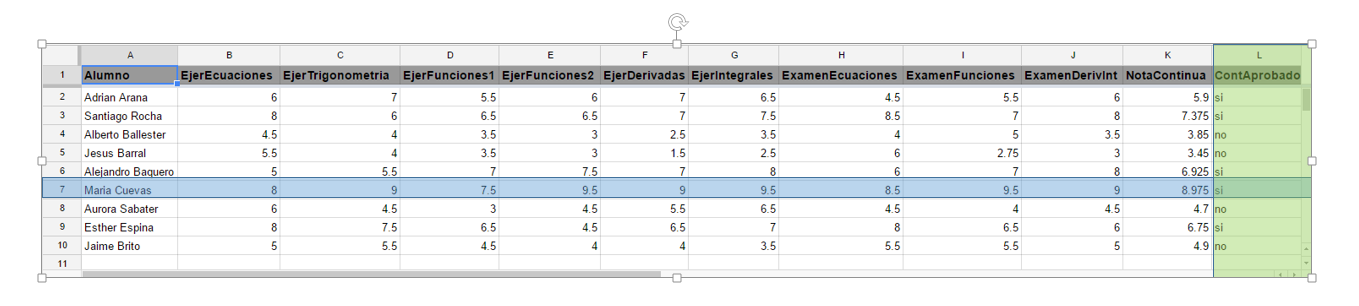
\includegraphics[width=1.1\textwidth]{./figs/SheetFilter.png}
	\caption{Funcionamiento de los filtros para realizar la búsqueda de la respuesta del chatbot en la hoja de cálculo.}
	\label{fig:SheetFilter}
\end{figure}

De igual manera se pueden realizar consultas enriquecidas, donde la entidad o el resultado fuesen un conjunto de más de una columna. Esto dependerá del dominio y de la representación de los datos. En los casos de estudio del Capítulo \ref{cha:CaseStudies} se profundiza más en qué tipo de consultas enriquecidas pueden definirse. Para realizar estas consultas se trabaja con un subconjunto de funciones de SQL, del que se puede profundizar en el Apartado \ref{sec:AlaSQL}. 

\subsubsection{Humanización}
\label{sec:Humanization}

La humanización de un chatbot consiste en hacer que un chatbot parezca más humano. Esto permite ofrecer una experiencia de usuario más próxima a una interacción con un humano real posible. Al fin y al cabo, un chatbot es un software y por muy humano que resulte, seguirá siendo un software, pero para un usuario no es lo mismo interactuar mediante comandos o mediante frases que le puedan salir de forma natural.

Para ello se ha trabajado en varios aspectos que permiten una experiencia de usuario más rica. Aunque se pueda mejorar, cabe recordar que el esfuerzo de humanizar conlleva un coste de tiempo de desarrollo. Si este coste es muy elevado, es posible que el usuario decida utilizar su aplicación de hojas de cálculo de toda la vida. Los cuatro aspectos en los que se ha hecho hincapié son los siguientes:
\begin{itemize}
	\item \textbf{Saludo}: Cada Chatbot ha de disponer de un mensaje de bienvenida o ayuda. Además de ser una buena práctica, este mensaje proporciona feedback (aunque sea a un nivel muy básico) de las funcionalidades que tiene el chatbot. Esto puede resultar útil a pesar de ser un chatbot para autoconsumo, ya que si se está un periodo largo de tiempo sin usarlo, se le podría olvidar al usuario en qué consistía ese chatbot.
	\item \textbf{Desambiguación del Intent}: tal y como se ha comentado en el Apartado \ref{sec:Queries} es necesario ser capaz de interpretar cuál es el Intent al que se refiere el usuario. Para ello se ha utilizado un servicio que mediante procesamiento del lenguaje natural desambiguar Intents y reconocer Entidades. En el Anexo \ref{anx:witai} hay más información acerca de este servicio denominado Wit.ai.
	\item \textbf{Sugerencias}: en una conversación puede surgir que el usuario al hacer una petición no haya introducido todas las Entidades que requiere el chatbot para proporcionar una respuesta. En estas situaciones el chatbot irá preguntando por cada una de las entidades que falten. Para mejorar la experiencia del usuario, el chatbot proporcionará sugerencias sobre posibles valores que hay registrados en la base de datos.
	\item \textbf{Personalización de la respuesta}: al trabajar con hojas de cálculo, el resultado de las consultas son celdas con un dato o un conjunto de datos concreto. A la hora de visualizar eso en una aplicación de mensajería instantánea resulta farragoso y bastante robótico. Es por eso, que se pueden definir frases que se completan con la respuesta que extraída de la hoja de cálculo. Es una técnica sencilla y que ayuda a una interpretación de la información más rápida.
\end{itemize}

\section{Modelo de datos}
\label{sec:DataModel}

Todas las características presentadas en el Apartado \ref{sec:FeatureModel} se han de representar en un modelo de datos. En este apartado en primer lugar se presentará el metamodelo y después la sintaxis concreta que será la que el motor de SheetChat interprete para generar el bot.

\subsection{Metamodelo}
\label{sec:Metamodel}

En la Figura \ref{fig:Metamodel} se puede observar cual es el Metamodelo definido para los chatbots generados por SheetChat. Un \textbf{SheetChat} consta de uno o más Sheets (u hojas de cálculo) y de un Chat.

Un \textbf{Sheet} está representado por un nombre de la hoja de cálculo, que debe de ser único, y el rango de los datos que conforman los datos que se quieren consultar.

Un \textbf{Chat} contiene una descripción del chatbot y un mensaje de saludo. El mensaje de saludo puede ser cualquier contenido textual, aunque como se ha mencionado en el Apartado \ref{sec:Humanization}, cuanto más descriptivo sea, mejor.

Un Chat contiene uno o más Intents. Cada \textbf{Intent} estará asociado a una hoja de cálculo donde deberá de buscar los datos, y contiene un identificador único, que será el que se defina en el entrenamiento de Wit.ai \ref{anx:witai}.

De igual manera un Intent está conformado por una o más Entity. Cada \textbf{Entity} tendrá que estar asociada a una o más columnas de la hoja de cálculo. El \emph{Mask} de una Entity define el tipo de comparación que se debe de hacer con el valor de las columnas. Del Mask dependerá el filtrado que se aplica a una fila concreta. Para los valores de tipo String se pueden utilizar el ``='' o el ``LIKE'', mientras que para los valores númericos se pueden hacer comparaciones de mayor, menor, mayor o igual, distinto de, etc. Las Entity permiten definir un mensaje personalizado para las preguntas que el chatbot puede hacer el usuario para recabar información acerca de la Entity a consultar. El \emph{entityMissingMsg} es un mensaje que se muestra si no se ha encontrado en la pregunta inicial la entidad requerida. El \emph{entityNotFoundMsg} hace referencia al caso donde el usuario ha proporcionado un valor para la entidad pero esta no se ha encontrado en la hoja de cálculo.

Por otro lado, un Intent tiene asociada una Response. Una \textbf{Response} consta de una o un conjunto de columnas o una columna extraida a partir de una fórmula matemática. El resto de parametros son opcionales. El numero de respuestas indica el número máximo de respuestas que puede dar el chatbot para esa respuesta. Es una funcionalidad útil si el filtrado genera muchas respuestas. \emph{CustomResponseStructure} permite definir una respuesta con un texto personalizado que hace más amena su lectura. El \emph{showColumnName} se puede utilizar en caso de que no se use el CustomResponseStructure. Esta se encarga de mostrar el nombre de la columna junto al valor de la celda respuesta. \emph{NotFoundMessage} es un mensaje personalizado que se muestra al usuario en caso de que no se hayan encontrado resultados.

\begin{figure}[htb]
	\centering
	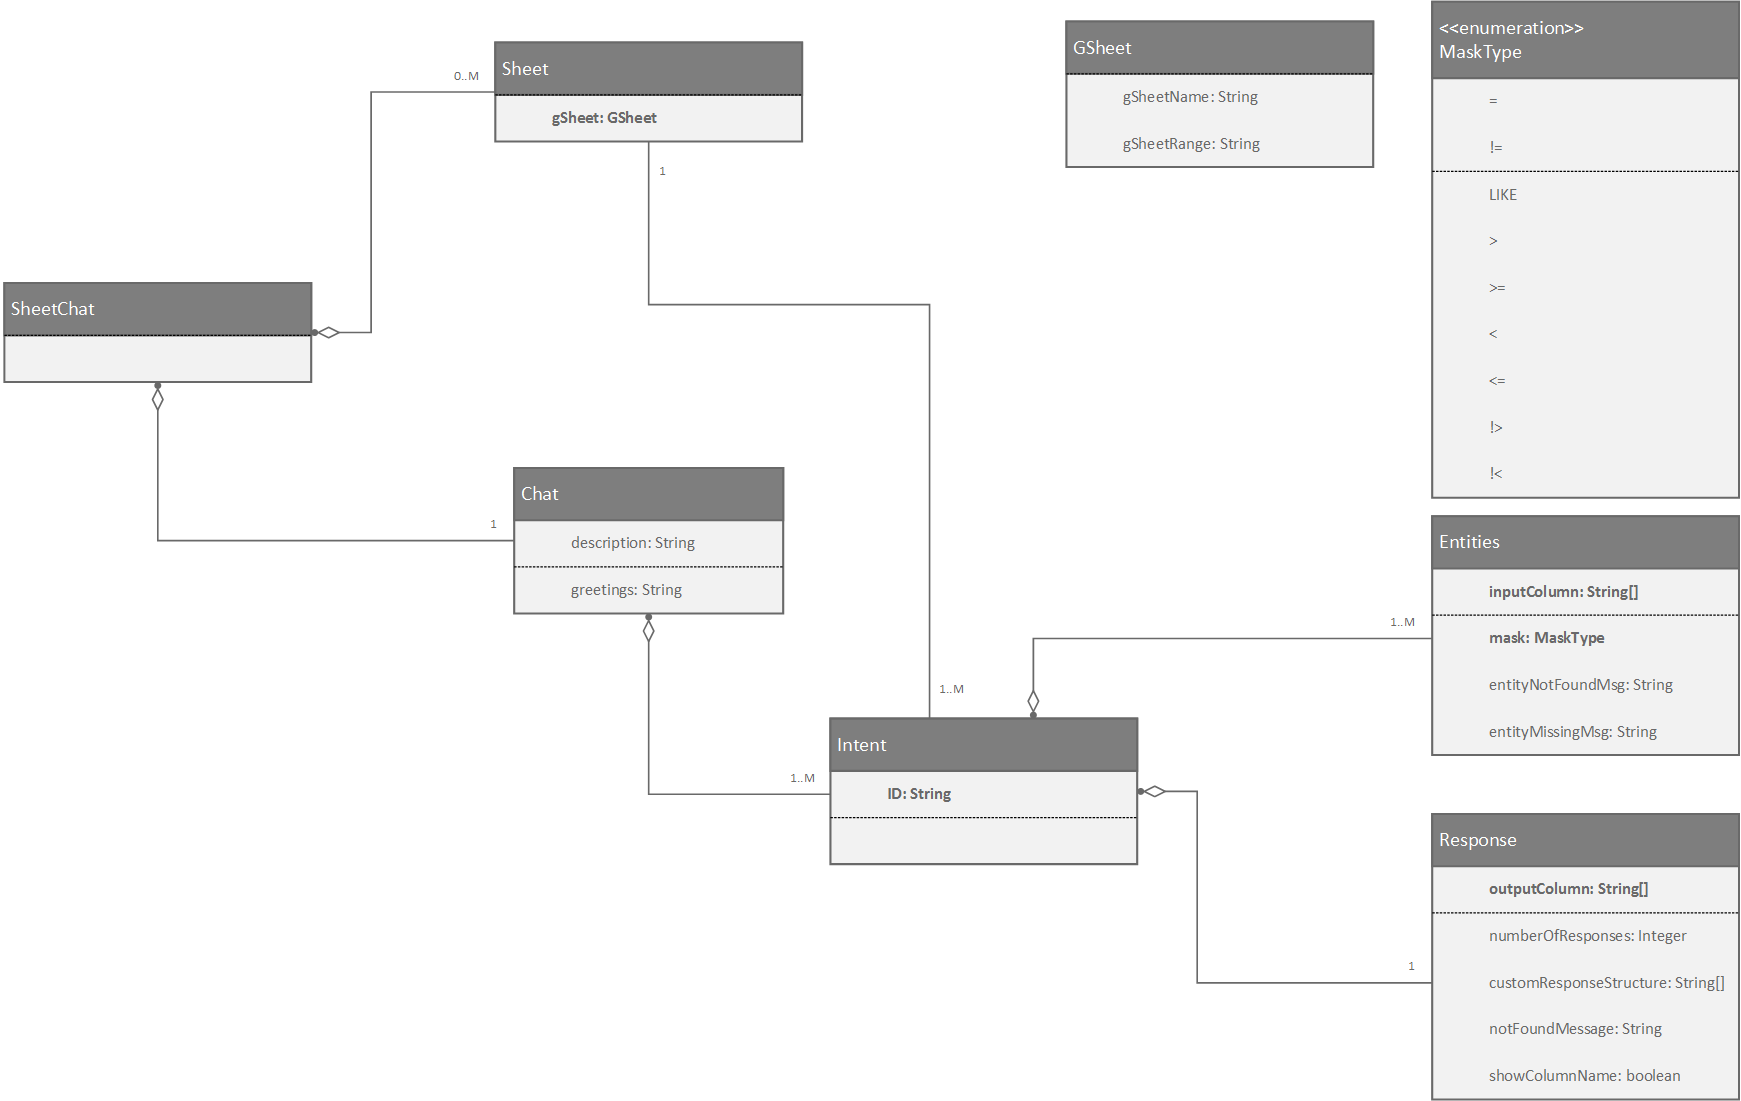
\includegraphics[width=1.1\textwidth]{./figs/Metamodel.png}
	\caption{Modelo de características de SheetChat.}
	\label{fig:Metamodel}
\end{figure}

\subsection{Sintaxis concreta}
\label{sec:ConcreteSyntax}

La sintaxis concreta está desarrollada en JSON. Entre los requisitos definidos, era conveniente que se utilizase un DSL definido en un lenguaje de fácil lectura y modificación por parte de un humano y sin duda JSON es de los mejores lenguajes para ello.

En la Figura \ref{fig:ConcreteSyntax} se observa la sintaxis concreta del caso de estudio descrito en el Apartado \ref{sec:EjemploNotas}

\begin{figure}[htb]
	\centering
	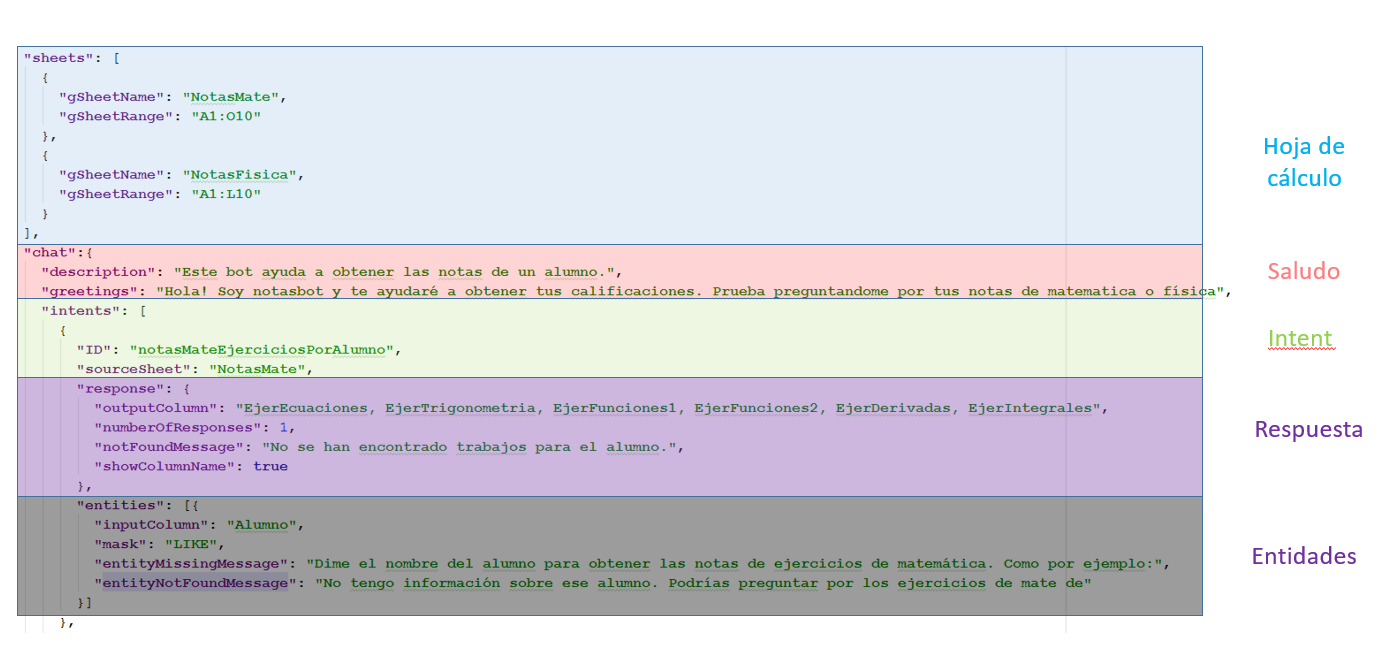
\includegraphics[width=1.1\textwidth]{./figs/DSLNotas.png}
	\caption{DSL con la definición de las Sheet y un Intent con una Entity.}
	\label{fig:ConcreteSyntax}
\end{figure}
